\documentclass{article}
\usepackage{tikz}
\usetikzlibrary{matrix,decorations,arrows,shapes,automata,backgrounds,fit,calc,petri,patterns,positioning}

\begin{document}

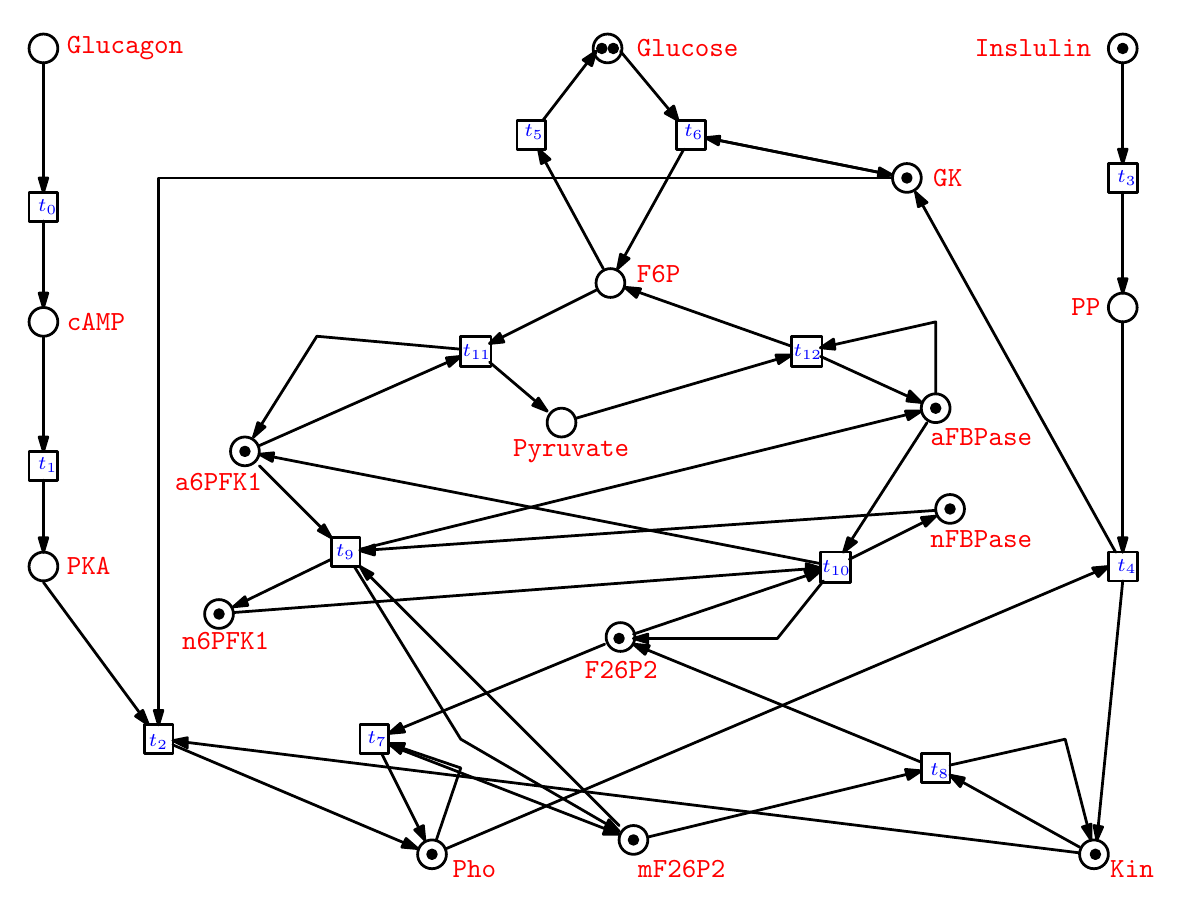
\begin{tikzpicture}[x=1pt,y=-1pt, scale=0.52]

\definecolor{BLACK}{RGB}{0,0,0}
\definecolor{WHITE}{RGB}{255,255,255}
\draw[BLACK, solid, line join=round, line cap=round, line width=1, fill=WHITE]
	(130,110) ellipse[x radius=10, y radius=10];
\draw[BLACK]
	(140,110) node[rotate=0, font=\ttfamily\normalsize, BLACK, right=-.25]
	{\textcolor{red}{Glucagon}};
\draw[BLACK, solid, line join=round, line cap=round, line width=1, fill=WHITE]
	(522,110) ellipse[x radius=10, y radius=10];
\draw[BLACK]
	(536,110) node[rotate=0, font=\ttfamily\normalsize, BLACK, right=-.25]
	{\textcolor{red}{Glucose}};
\draw[BLACK, solid, line join=round, line cap=round, line width=1, fill=BLACK]
	(518,110) ellipse[x radius=3, y radius=3];
\draw[BLACK, solid, line join=round, line cap=round, line width=1, fill=BLACK]
	(526,110) ellipse[x radius=3, y radius=3];
\draw[BLACK, solid, line join=round, line cap=round, line width=1, fill=WHITE]
	(880,110) ellipse[x radius=10, y radius=10];
\draw[BLACK]
	(771,110) node[rotate=0, font=\ttfamily\normalsize, BLACK, right=-.25]
	{\textcolor{red}{Inslulin}};
\draw[BLACK, solid, line join=round, line cap=round, line width=1, fill=BLACK]
	(880,110) ellipse[x radius=3, y radius=3];
\draw[BLACK, solid, line join=round, line cap=round, line width=1, fill=WHITE]
	(130,300) ellipse[x radius=10, y radius=10];
\draw[BLACK]
	(140,300) node[rotate=0, font=\ttfamily\normalsize, BLACK, right=-.25]
	{\textcolor{red}{cAMP}};
\draw[BLACK, solid, line join=round, line cap=round, line width=1, fill=WHITE]
	(130,470) ellipse[x radius=10, y radius=10];
\draw[BLACK]
	(140,470) node[rotate=0, font=\ttfamily\normalsize, BLACK, right=-.25]
	{\textcolor{red}{PKA}};
\draw[BLACK, solid, line join=round, line cap=round, line width=1, fill=WHITE]
	(400,670) ellipse[x radius=10, y radius=10];
\draw[BLACK]
	(408,680) node[rotate=0, font=\ttfamily\normalsize, BLACK, right=-.25]
	{\textcolor{red}{Pho}};
\draw[BLACK, solid, line join=round, line cap=round, line width=1, fill=BLACK]
	(400,670) ellipse[x radius=3, y radius=3];
\draw[BLACK, solid, line join=round, line cap=round, line width=1, fill=WHITE]
	(860,670) ellipse[x radius=10, y radius=10];
\draw[BLACK]
	(865,680) node[rotate=0, font=\ttfamily\normalsize, BLACK, right=-.25]
	{\textcolor{red}{Kin}};
\draw[BLACK, solid, line join=round, line cap=round, line width=1, fill=BLACK]
	(861,670) ellipse[x radius=3, y radius=3];
\draw[BLACK, solid, line join=round, line cap=round, line width=1, fill=WHITE]
	(880,290) ellipse[x radius=10, y radius=10];
\draw[BLACK]
	(838,290) node[rotate=0, font=\ttfamily\normalsize, BLACK, right=-.25]
	{\textcolor{red}{PP}};
\draw[BLACK, solid, line join=round, line cap=round, line width=1, fill=WHITE]
	(730,200) ellipse[x radius=10, y radius=10];
\draw[BLACK]
	(742,200) node[rotate=0, font=\ttfamily\normalsize, BLACK, right=-.25]
	{\textcolor{red}{GK}};
\draw[BLACK, solid, line join=round, line cap=round, line width=1, fill=BLACK]
	(730,200) ellipse[x radius=3, y radius=3];
\draw[BLACK, solid, line join=round, line cap=round, line width=1, fill=WHITE]
	(524,273) ellipse[x radius=10, y radius=10];
\draw[BLACK]
	(536,267) node[rotate=0, font=\ttfamily\normalsize, BLACK, right=-.25]
	{\textcolor{red}{F6P}};
\draw[BLACK, solid, line join=round, line cap=round, line width=1, fill=WHITE]
	(531,519) ellipse[x radius=10, y radius=10];
\draw[BLACK]
	(500,542) node[rotate=0, font=\ttfamily\normalsize, BLACK, right=-.25]
	{\textcolor{red}{F26P2}};
\draw[BLACK, solid, line join=round, line cap=round, line width=1, fill=BLACK]
	(530,520) ellipse[x radius=3, y radius=3];
\draw[BLACK, solid, line join=round, line cap=round, line width=1, fill=WHITE]
	(270,390) ellipse[x radius=10, y radius=10];
\draw[BLACK]
	(215,411) node[rotate=0, font=\ttfamily\normalsize, BLACK, right=-.25]
	{\textcolor{red}{a6PFK1}};
\draw[BLACK, solid, line join=round, line cap=round, line width=1, fill=BLACK]
	(270,390) ellipse[x radius=3, y radius=3];
\draw[BLACK, solid, line join=round, line cap=round, line width=1, fill=WHITE]
	(252,503) ellipse[x radius=10, y radius=10];
\draw[BLACK]
	(220,522) node[rotate=0, font=\ttfamily\normalsize, BLACK, right=-.25]
	{\textcolor{red}{n6PFK1}};
\draw[BLACK, solid, line join=round, line cap=round, line width=1, fill=BLACK]
	(252,503) ellipse[x radius=3, y radius=3];
\draw[BLACK, solid, line join=round, line cap=round, line width=1, fill=WHITE]
	(750,360) ellipse[x radius=10, y radius=10];
\draw[BLACK]
	(740,380) node[rotate=0, font=\ttfamily\normalsize, BLACK, right=-.25]
	{\textcolor{red}{aFBPase}};
\draw[BLACK, solid, line join=round, line cap=round, line width=1, fill=BLACK]
	(750,360) ellipse[x radius=3, y radius=3];
\draw[BLACK, solid, line join=round, line cap=round, line width=1, fill=WHITE]
	(760,430) ellipse[x radius=10, y radius=10];
\draw[BLACK]
	(740,451) node[rotate=0, font=\ttfamily\normalsize, BLACK, right=-.25]
	{\textcolor{red}{nFBPase}};
\draw[BLACK, solid, line join=round, line cap=round, line width=1, fill=BLACK]
	(760,430) ellipse[x radius=3, y radius=3];
\draw[BLACK, solid, line join=round, line cap=round, line width=1, fill=WHITE]
	(490,370) ellipse[x radius=10, y radius=10];
\draw[BLACK]
	(450,390) node[rotate=0, font=\ttfamily\normalsize, BLACK, right=-.25]
	{\textcolor{red}{Pyruvate}};
\draw[BLACK, solid, line join=round, line cap=round, line width=1, fill=WHITE]
	(540,660) ellipse[x radius=10, y radius=10];
\draw[BLACK]
	(537,680) node[rotate=0, font=\ttfamily\normalsize, BLACK, right=-.25]
	{\textcolor{red}{mF26P2}};
\draw[BLACK, solid, line join=round, line cap=round, line width=1, fill=BLACK]
	(540,660) ellipse[x radius=3, y radius=3];
\draw[BLACK, solid, line join=round, line cap=round, line width=1, fill=WHITE]
	(120,210) rectangle +(20,20);
\draw[BLACK]
	(120,220) node[rotate=0, font=\ttfamily\normalsize, BLACK, right=-.25]
	{\textcolor{blue}{\scriptsize{$t_0$}}};
\draw[BLACK, solid, line join=round, line cap=round, line width=1, fill=WHITE]
	(120,390) rectangle +(20,20);
\draw[BLACK]
	(120,399.5) node[rotate=0, font=\ttfamily\normalsize, BLACK, right=-.25]
	{\textcolor{blue}{\scriptsize{$t_1$}}};
\draw[BLACK, solid, line join=round, line cap=round, line width=1, fill=WHITE]
	(200,580) rectangle +(20,20);
\draw[BLACK]
	(197,592) node[rotate=0, font=\ttfamily\normalsize, BLACK, right=-.25]
	{\textcolor{blue}{\scriptsize{$t_2$}}};
\draw[BLACK, solid, line join=round, line cap=round, line width=1, fill=WHITE]
	(870,190) rectangle +(20,20);
\draw[BLACK]
	(870,200) node[rotate=0, font=\ttfamily\normalsize, BLACK, right=-.25]
	{\textcolor{blue}{\scriptsize{$t_3$}}};
\draw[BLACK, solid, line join=round, line cap=round, line width=1, fill=WHITE]
	(870,460) rectangle +(20,20);
\draw[BLACK]
	(870,470) node[rotate=0, font=\ttfamily\normalsize, BLACK, right=-.25]
	{\textcolor{blue}{\scriptsize{$t_4$}}};
\draw[BLACK, solid, line join=round, line cap=round, line width=1, fill=WHITE]
	(570,160) rectangle +(20,20);
\draw[BLACK]
	(569,168) node[rotate=0, font=\ttfamily\normalsize, BLACK, right=-.25]
	{\textcolor{blue}{\scriptsize{$t_6$}}};
\draw[BLACK, solid, line join=round, line cap=round, line width=1, fill=WHITE]
	(459,160) rectangle +(20,20);
\draw[BLACK]
	(458,168) node[rotate=0, font=\ttfamily\normalsize, BLACK, right=-.25]
	{\textcolor{blue}{\scriptsize{$t_5$}}};
\draw[BLACK, solid, line join=round, line cap=round, line width=1, fill=WHITE]
	(350,580) rectangle +(20,20);
\draw[BLACK]
	(349,590) node[rotate=0, font=\ttfamily\normalsize, BLACK, right=-.25]
	{\textcolor{blue}{\scriptsize{$t_7$}}};
\draw[BLACK, solid, line join=round, line cap=round, line width=1, fill=WHITE]
	(740,600) rectangle +(20,20);
\draw[BLACK]
	(740,612) node[rotate=0, font=\ttfamily\normalsize, BLACK, right=-.25]
	{\textcolor{blue}{\scriptsize{$t_8$}}};
\draw[BLACK, solid, line join=round, line cap=round, line width=1, fill=WHITE]
	(330,450) rectangle +(20,20);
\draw[BLACK]
	(327,460) node[rotate=0, font=\ttfamily\normalsize, BLACK, right=-.25]
	{\textcolor{blue}{\scriptsize{$t_9$}}};
\draw[BLACK, solid, line join=round, line cap=round, line width=1, fill=WHITE]
	(670,460) rectangle +(21,21);
\draw[BLACK]
	(665,471) node[rotate=0, font=\ttfamily\normalsize, BLACK, right=-.25]
	{\textcolor{blue}{\scriptsize{$t_{10}$}}};
\draw[BLACK, solid, line join=round, line cap=round, line width=1, fill=WHITE]
	(420,310) rectangle +(21,21);
\draw[BLACK]
	(415,321) node[rotate=0, font=\ttfamily\normalsize, BLACK, right=-.25]
	{\textcolor{blue}{\scriptsize{$t_{11}$}}};
\draw[BLACK, solid, line join=round, line cap=round, line width=1, fill=WHITE]
	(650,310) rectangle +(21,21);
\draw[BLACK]
	(645,321) node[rotate=0, font=\ttfamily\normalsize, BLACK, right=-.25]
	{\textcolor{blue}{\scriptsize{$t_{12}$}}};
\draw[BLACK, solid, line join=round, line cap=round, line width=1]
	(130,120) -- (130,210);
\draw[BLACK, solid, line join=round, line cap=round, line width=1, fill=BLACK]
	(130,210) -- (127,200) -- (133,200) -- (130,210) -- cycle;
\draw[BLACK, solid, line join=round, line cap=round, line width=1]
	(130,230) -- (130,290);
\draw[BLACK, solid, line join=round, line cap=round, line width=1, fill=BLACK]
	(127,280) -- (133,280) -- (130,290) -- (127,280) -- cycle;
\draw[BLACK, solid, line join=round, line cap=round, line width=1]
	(130,310) -- (130,390);
\draw[BLACK, solid, line join=round, line cap=round, line width=1, fill=BLACK]
	(127,380) -- (133,380) -- (130,390) -- (127,380) -- cycle;
\draw[BLACK, solid, line join=round, line cap=round, line width=1]
	(130,410) -- (130,460);
\draw[BLACK, solid, line join=round, line cap=round, line width=1, fill=BLACK]
	(127,450) -- (133,450) -- (130,460) -- (127,450) -- cycle;
\draw[BLACK, solid, line join=round, line cap=round, line width=1]
	(130,481) -- (203,580);
\draw[BLACK, solid, line join=round, line cap=round, line width=1, fill=BLACK]
	(203,580) -- (194,574) -- (199,570) -- (203,580) -- cycle;
\draw[BLACK, solid, line join=round, line cap=round, line width=1]
	(220,594) -- (390,666);
\draw[BLACK, solid, line join=round, line cap=round, line width=1, fill=BLACK]
	(390,666) -- (379,665) -- (382,659) -- (390,666) -- cycle;
\draw[BLACK, solid, line join=round, line cap=round, line width=1]
	(850,669) -- (220,591);
\draw[BLACK, solid, line join=round, line cap=round, line width=1, fill=BLACK]
	(220,591) -- (230,589) -- (230,596) -- (220,591) -- cycle;
\draw[BLACK, solid, line join=round, line cap=round, line width=1]
	(880,120) -- (880,190);
\draw[BLACK, solid, line join=round, line cap=round, line width=1, fill=BLACK]
	(880,190) -- (877,180) -- (883,180) -- (880,190) -- cycle;
\draw[BLACK, solid, line join=round, line cap=round, line width=1]
	(880,210) -- (880,280);
\draw[BLACK, solid, line join=round, line cap=round, line width=1, fill=BLACK]
	(877,270) -- (883,270) -- (880,280) -- (877,270) -- cycle;
\draw[BLACK, solid, line join=round, line cap=round, line width=1]
	(880,300) -- (880,460);
\draw[BLACK, solid, line join=round, line cap=round, line width=1, fill=BLACK]
	(877,450) -- (883,450) -- (880,460) -- (877,450) -- cycle;
\draw[BLACK, solid, line join=round, line cap=round, line width=1]
	(880,480) -- (862,660);
\draw[BLACK, solid, line join=round, line cap=round, line width=1, fill=BLACK]
	(862,660) -- (860,650) -- (866,651) -- (862,660) -- cycle;
\draw[BLACK, solid, line join=round, line cap=round, line width=1]
	(410,666) -- (870,470);
\draw[BLACK, solid, line join=round, line cap=round, line width=1, fill=BLACK]
	(870,470) -- (863,477) -- (859,471) -- (870,470) -- cycle;
\draw[BLACK, solid, line join=round, line cap=round, line width=1]
	(531,112) -- (571,160);
\draw[BLACK, solid, line join=round, line cap=round, line width=1, fill=BLACK]
	(571,160) -- (562,155) -- (568,150) -- (571,160) -- cycle;
\draw[BLACK, solid, line join=round, line cap=round, line width=1]
	(850,665) -- (760,615);
\draw[BLACK, solid, line join=round, line cap=round, line width=1, fill=BLACK]
	(760,615) -- (770,617) -- (767,623) -- (760,615) -- cycle;
\draw[BLACK, solid, line join=round, line cap=round, line width=1]
	(365,600) -- (395,660);
\draw[BLACK, solid, line join=round, line cap=round, line width=1, fill=BLACK]
	(395,660) -- (388,653) -- (394,650) -- (395,660) -- cycle;
\draw[BLACK, solid, line join=round, line cap=round, line width=1]
	(403,660) -- (420,610) -- (370,593);
\draw[BLACK, solid, line join=round, line cap=round, line width=1, fill=BLACK]
	(370,593) -- (381,593) -- (378,600) -- (370,593) -- cycle;
\draw[BLACK, solid, line join=round, line cap=round, line width=1]
	(760,608) -- (840,590) -- (858,660);
\draw[BLACK, solid, line join=round, line cap=round, line width=1, fill=BLACK]
	(858,660) -- (852,651) -- (858,649) -- (858,660) -- cycle;
\draw[BLACK, solid, line join=round, line cap=round, line width=1]
	(477,160) -- (514,112);
\draw[BLACK, solid, line join=round, line cap=round, line width=1, fill=BLACK]
	(514,112) -- (511,122) -- (505,118) -- (514,112) -- cycle;
\draw[BLACK, solid, line join=round, line cap=round, line width=1]
	(520,524) -- (370,586);
\draw[BLACK, solid, line join=round, line cap=round, line width=1, fill=BLACK]
	(370,586) -- (378,579) -- (381,585) -- (370,586) -- cycle;
\draw[BLACK, solid, line join=round, line cap=round, line width=1]
	(740,606) -- (540,524);
\draw[BLACK, solid, line join=round, line cap=round, line width=1, fill=BLACK]
	(540,524) -- (551,525) -- (548,531) -- (540,524) -- cycle;
\draw[BLACK, solid, line join=round, line cap=round, line width=1]
	(280,400) -- (330,450);
\draw[BLACK, solid, line join=round, line cap=round, line width=1, fill=BLACK]
	(330,450) -- (321,445) -- (325,441) -- (330,450) -- cycle;
\draw[BLACK, solid, line join=round, line cap=round, line width=1]
	(330,465) -- (262,498);
\draw[BLACK, solid, line join=round, line cap=round, line width=1, fill=BLACK]
	(262,498) -- (270,491) -- (272,497) -- (262,498) -- cycle;
\draw[BLACK, solid, line join=round, line cap=round, line width=1]
	(750,431) -- (350,459);
\draw[BLACK, solid, line join=round, line cap=round, line width=1, fill=BLACK]
	(350,459) -- (360,455) -- (360,462) -- (350,459) -- cycle;
\draw[BLACK, solid, line join=round, line cap=round, line width=1]
	(350,458) -- (740,362);
\draw[BLACK, solid, line join=round, line cap=round, line width=1, fill=BLACK]
	(740,362) -- (731,368) -- (729,362) -- (740,362) -- cycle;
\draw[BLACK, solid, line join=round, line cap=round, line width=1]
	(670,468) -- (280,392);
\draw[BLACK, solid, line join=round, line cap=round, line width=1, fill=BLACK]
	(280,392) -- (290,391) -- (289,397) -- (280,392) -- cycle;
\draw[BLACK, solid, line join=round, line cap=round, line width=1]
	(262,502) -- (670,471);
\draw[BLACK, solid, line join=round, line cap=round, line width=1, fill=BLACK]
	(670,471) -- (660,475) -- (660,468) -- (670,471) -- cycle;
\draw[BLACK, solid, line join=round, line cap=round, line width=1]
	(744,370) -- (686,460);
\draw[BLACK, solid, line join=round, line cap=round, line width=1, fill=BLACK]
	(686,460) -- (689,450) -- (695,453) -- (686,460) -- cycle;
\draw[BLACK, solid, line join=round, line cap=round, line width=1]
	(690,465) -- (750,435);
\draw[BLACK, solid, line join=round, line cap=round, line width=1, fill=BLACK]
	(750,435) -- (743,442) -- (740,436) -- (750,435) -- cycle;
\draw[BLACK, solid, line join=round, line cap=round, line width=1]
	(514,278) -- (440,315);
\draw[BLACK, solid, line join=round, line cap=round, line width=1, fill=BLACK]
	(440,315) -- (447,308) -- (450,314) -- (440,315) -- cycle;
\draw[BLACK, solid, line join=round, line cap=round, line width=1]
	(440,328) -- (480,362);
\draw[BLACK, solid, line join=round, line cap=round, line width=1, fill=BLACK]
	(480,362) -- (470,358) -- (474,353) -- (480,362) -- cycle;
\draw[BLACK, solid, line join=round, line cap=round, line width=1]
	(280,386) -- (420,324);
\draw[BLACK, solid, line join=round, line cap=round, line width=1, fill=BLACK]
	(420,324) -- (412,331) -- (410,325) -- (420,324) -- cycle;
\draw[BLACK, solid, line join=round, line cap=round, line width=1]
	(420,319) -- (320,310) -- (276,380);
\draw[BLACK, solid, line join=round, line cap=round, line width=1, fill=BLACK]
	(276,380) -- (279,370) -- (284,373) -- (276,380) -- cycle;
\draw[BLACK, solid, line join=round, line cap=round, line width=1]
	(750,350) -- (750,300) -- (670,318);
\draw[BLACK, solid, line join=round, line cap=round, line width=1, fill=BLACK]
	(670,318) -- (679,312) -- (680,319) -- (670,318) -- cycle;
\draw[BLACK, solid, line join=round, line cap=round, line width=1]
	(670,324) -- (740,356);
\draw[BLACK, solid, line join=round, line cap=round, line width=1, fill=BLACK]
	(740,356) -- (730,355) -- (732,348) -- (740,356) -- cycle;
\draw[BLACK, solid, line join=round, line cap=round, line width=1]
	(500,367) -- (650,323);
\draw[BLACK, solid, line join=round, line cap=round, line width=1, fill=BLACK]
	(650,323) -- (641,329) -- (639,323) -- (650,323) -- cycle;
\draw[BLACK, solid, line join=round, line cap=round, line width=1]
	(650,317) -- (534,276);
\draw[BLACK, solid, line join=round, line cap=round, line width=1, fill=BLACK]
	(534,276) -- (545,277) -- (542,283) -- (534,276) -- cycle;
\draw[BLACK, solid, line join=round, line cap=round, line width=1]
	(550,658) -- (740,612);
\draw[BLACK, solid, line join=round, line cap=round, line width=1, fill=BLACK]
	(740,612) -- (731,618) -- (729,611) -- (740,612) -- cycle;
\draw[BLACK, solid, line join=round, line cap=round, line width=1]
	(370,594) -- (530,656);
\draw[BLACK, solid, line join=round, line cap=round, line width=1, fill=BLACK]
	(530,656) -- (519,656) -- (522,649) -- (530,656) -- cycle;
\draw[BLACK, solid, line join=round, line cap=round, line width=1]
	(530,650) -- (350,470);
\draw[BLACK, solid, line join=round, line cap=round, line width=1, fill=BLACK]
	(350,470) -- (359,475) -- (355,479) -- (350,470) -- cycle;
\draw[BLACK, solid, line join=round, line cap=round, line width=1]
	(346,470) -- (420,590) -- (530,654);
\draw[BLACK, solid, line join=round, line cap=round, line width=1, fill=BLACK]
	(530,654) -- (520,652) -- (523,646) -- (530,654) -- cycle;
\draw[BLACK, solid, line join=round, line cap=round, line width=1]
	(540,517) -- (670,473);
\draw[BLACK, solid, line join=round, line cap=round, line width=1, fill=BLACK]
	(670,473) -- (662,480) -- (659,473) -- (670,473) -- cycle;
\draw[BLACK, solid, line join=round, line cap=round, line width=1]
	(672,480) -- (640,520) -- (540,520);
\draw[BLACK, solid, line join=round, line cap=round, line width=1, fill=BLACK]
	(540,520) -- (550,517) -- (550,523) -- (540,520) -- cycle;
\draw[BLACK, solid, line join=round, line cap=round, line width=1]
	(875,460) -- (736,210);
\draw[BLACK, solid, line join=round, line cap=round, line width=1, fill=BLACK]
	(736,210) -- (744,217) -- (738,220) -- (736,210) -- cycle;
\draw[BLACK, solid, line join=round, line cap=round, line width=1]
	(590,172) -- (720,198);
\draw[BLACK, solid, line join=round, line cap=round, line width=1, fill=BLACK]
	(720,198) -- (710,199) -- (711,193) -- (720,198) -- cycle;
\draw[BLACK, solid, line join=round, line cap=round, line width=1]
	(720,198) -- (590,172);
\draw[BLACK, solid, line join=round, line cap=round, line width=1, fill=BLACK]
	(590,172) -- (600,171) -- (599,177) -- (590,172) -- cycle;
\draw[BLACK, solid, line join=round, line cap=round, line width=1]
	(720,200) -- (210,200) -- (210,580);
\draw[BLACK, solid, line join=round, line cap=round, line width=1, fill=BLACK]
	(210,580) -- (207,570) -- (213,570) -- (210,580) -- cycle;
\draw[BLACK, solid, line join=round, line cap=round, line width=1]
	(519,263) -- (474,180);
\draw[BLACK, solid, line join=round, line cap=round, line width=1, fill=BLACK]
	(474,180) -- (482,187) -- (476,190) -- (474,180) -- cycle;
\draw[BLACK, solid, line join=round, line cap=round, line width=1]
	(575,180) -- (529,263);
\draw[BLACK, solid, line join=round, line cap=round, line width=1, fill=BLACK]
	(529,263) -- (531,253) -- (537,256) -- (529,263) -- cycle;
\end{tikzpicture}

\end{document}